\documentclass[border = 0.2cm, 12pt]{standalone}
\usepackage{amsmath, amssymb, amsfonts}
\usepackage{xcolor}
\usepackage{tikz, pgfplots}
\pgfplotsset{compat=newest}
\usetikzlibrary{shapes, snakes, angles, quotes, arrows.meta}
\tikzset{>=latex}
\usetikzlibrary{angles,quotes}
\usepackage{tkz-euclide}

\usepackage{helvet}
\renewcommand{\familydefault}{\sfdefault}
\usepackage[eulergreek]{sansmath}

% Dark theme setup
\pagecolor{black!85} % Slightly softer black
\color{white} % Default text color

\begin{document}

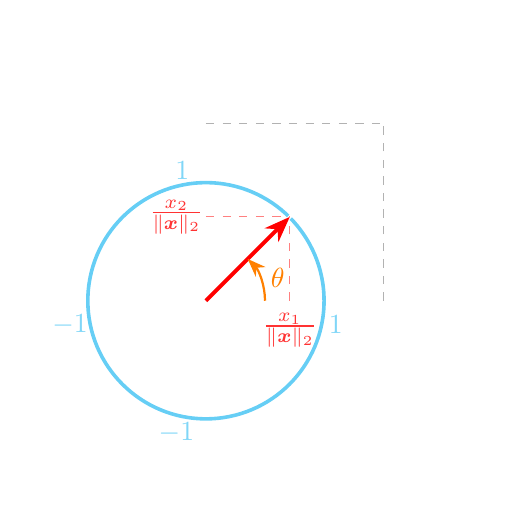
\begin{tikzpicture}[scale=1.5, >=Stealth, every node/.style={font=\sffamily}]

% Axes with labels
\draw[->, line width=0.8, white] (-1.5,0) -- (2,0) node[right] {$x$};
\draw[->, line width=0.8, white] (0,-1.5) -- (0,2) node[above] {$y$};

% Unit circle (drawn first to be in background)
\draw[fill=none, color=cyan!60, line width=1.3] (0,0) circle (1);

% Main vector and projections
\draw[arrows=->, line width=1.2, white] (0,0)--(1.5,1.5);
\draw[dashed, color=gray!60, thin] (1.5,0) -- (1.5,1.5) node[pos=0.5, right, color=white] {$x_2$};
\draw[dashed, color=gray!60, thin] (0,1.5) -- (1.5,1.5) node[pos=0.5, above, color=white] {$x_1$};
\node[color=white] at (1.6,1.6) {$\boldsymbol{x}$};

% Normalized vector and projections
\draw[arrows=->, line width=1.4, color=red] (0,0)--(0.71,0.71);
\draw[dashed, color=red!50, thin] (0.71,0)--(0.71,0.71);
\draw[dashed, color=red!50, thin] (0,0.71)--(0.71,0.71);
\node[color=red!80] at (0.71,-0.25) {$\frac{x_1}{\|\boldsymbol{x}\|_2}$};
\node[color=red!80] at (-0.25,0.71) {$\frac{x_2}{\|\boldsymbol{x}\|_2}$};

\node[color=cyan!50] at (1.1,-0.2) {$1$};
\node[color=cyan!50] at (-1.15,-0.2) {$-1$};
\node[color=cyan!50] at (-0.2,1.1) {$1$};
\node[color=cyan!50] at (-0.25,-1.12) {$-1$};

% Angle arc
\draw[color=orange, thick, ->] (0.5,0) arc (0:45:0.5) node[midway, right, color=orange] {$\theta$};

\end{tikzpicture}

\end{document}
